% Created 2024-12-08 Sun 22:14
% Intended LaTeX compiler: pdflatex
\documentclass[11pt]{article}

\input{../../../preamble.tex}
% setting up title page
\title{
  
\includegraphics[width=0.4\textwidth]{fmf_logo}\\
  {\small Oddelek za fiziko} \\
  {Hallov pojav}\\
  {\small Poročilo pri FP5}\\

}
\date{}
\author{ Kristofer Č. Povšič, 28211104 \\[5 cm]
 \small  Asistent: Tilen Knaflič \\
}
\begin{document}

\maketitle
\newpage
\tableofcontents
\newpage

\section{Uvod}\label{sec:org4245ae2}

\subsection{Hallov pojav}\label{sec:orgfbbc1a9}

Hallov pojav je pojav napetosti v prevodniku v smeri \(y\), če skozi prevodnik v smeri \(x\) teče tok ter je prevodnik postavljen v magnetno polje v smeri \(z\). Ta napetost uravnovesi magnetno silo na gibajoče se elektrone.

Prevodnik z dolžino \(a\) v smeri \(x\), s širino \(b\) v smeri \(y\) ter z višino \(c\) v smeri \(z\) postavimo v magnetno polje. Skozi prevodnik teče tok in predpostavimo, da so nosilci naboja elektroni z nabojem \(-e_0\). Gostota toka \(j = \frac{I}{bc}\) je za elektrone podana tudi z \(j = - ne_0v\), kjer sta \(n\) in \(v\) gostota in hitrost nosilcev naboja.

Elektroni se zaradi magnetne sile \(F_m = - e_0v B\), ki deluje v smeri \(-y\) začnejo kopičiti na robu prevodnika. Tako se na nasprotnih smereh robov prevodnika nabereta nasprotna naboja. Dobimo prečno napetost \(E_y\) v smeri \(-y\) ter električno silo \(F_2 = -e_0 (-E_y) = e_0E_y\), ki uravnovesi magnetno silo.

Po vzpostavitvi ravnovesja, kjer velja \(F_m + F_e = 0\) dobimo izraz za Hallovo napetost

\begin{equation}
\label{eq:1}
U_H = E_y b = - \frac{jBb}{ne_0} = - \frac{I B}{ne_0 c}
\end{equation}

Kvocient \(\frac{E_y}{jB}\) imenujemo Hallova konstanta in ga označimoz \(R_H\). Lahko jo tudi izrazimo kot

\begin{equation}
\label{eq:2}
R_H = - \frac{1}{ne_0} = \frac{U_H c}{IB}
\end{equation}

Iz enačbe \ref{eq:1} sledi, da lahko Hallov pojav uporabimo za merjenje gostote magnetnega polja \(B\). Skozi Hallovo sondo, ki je bila umerjena v znanem magnetnem polju pošljemo isti električni tok in tako lahko izmerimo \(B\). Iz enačbe \ref{eq:2} pa sledi, da lahko z merjenjem Hallove konstante določimo predznak in gostoto nosilcev naboja v raznih materialih, kar bomo pri tej vaji tudi počeli.
\subsection{Polprevodniki}\label{sec:org1c9d802}
Kristal z \(N\) atomi ima \(N\) energijskih nivojev kot posledici prekrivanja atomskih orbital. Kristal je izolator, če ima do neke energije vse energijske pasove polne, ostali pa so prazni in ločeni z dovolj širokim prepovedanim pasom.

V prevodniku je najvišje ležeči neprazni energijski pas le delno zaseden. Elektroni tako prejmejo kinetično energijo, ko se gibljejo v električnem polju. 

Če je energijska reža prepovedanega pasu \(1 \mathrm{eV}\), lahko pri dovolj visoki temperaturi del elektronov preide v prevodni pas in s tem prevaja električni tok - govorimo o polprevodnikih.

Če polprevodniku primešamo nečistoče v obliki petvalentnih elektronov, imajo primesi en odvečni elektron. Potrebuje zelo nizko energijo, da preskoči v prevodni pas. Temu dodatnemu nivoju rečemo donorski pas in ima energijo \(E_d\) in leži tik po prevodnim pasom. Večinski nosilci naboja so elektroni in zato mu rečemo polprevodnik tipa n. Če so večinski nosilci naboja vrzeli, primes je trivalentni atom, pa govorimo o polprevodniku tipa p.  

H gostoti elektronov v prevodnem pasu pri polprevodniku n prispevajo tudi termično dvignjeni elektroni iz donorskega pasu, lahko preko merjenja Hallove napetosti izmerimo temperaturno odvisnost gostote nosilcev naboja.
\subsection{Eksperiment}\label{sec:orgb97d12e}
Izmerimo Hallovo napetost \(U_H\) pri znani vrednosti polja \(B\), debeline vzorca germanija \(c\) in znanem toku \(I\) skozi vzorec. Iz tega izračunamo tudi Hallovo konstanto \(R_H\). Na temperaturnem območju \([20 ^{\circ}, 80^{\circ}]\) se občutno spremeni razmerje med donorskimi in valenčnimi elektroni v prevodnem pasu.

Če narišemo graf \(\ln n_p (\frac{1}{k_B T})\), dobimo pri nizkih temperaturah premico z naklonom \(- \frac{1}{2} E_g\), potem konstanto in nato naklon premice \(- \frac{1}{2}E_d\). Pri našem germaniju sta vrednosti \(E_g = 0.66eV\) in \(E_d \approx 0.01 eV\).
\section{Pripomočki}\label{sec:org054ebb6}
\begin{itemize}
\item Vzorec germanijevega polprevodnika tipa n s pripravljeno vezavo na kontakte
\item izolirano posodo olja z grelcem, mešalcem in magnetom
\item napajalnik za grelec in mešalec
\item digitalni voltmeter
\item digitalni ampermeter
\item termometer
\end{itemize}

\section{Naloge}\label{sec:org46b2437}
\begin{itemize}
\item izmeri temperaturno odvisnost Hallove napetosti vzorca polprevodnika tipa n na temperaturnem območju \([20^{\circ}, 80^{\circ}]\).
\item nariši graf ohmske upornosti \(R\) v odvisnosti od temperature \(T\)
\item nariši graf Hallove konstante \(R_H\) v odvisnost od temperature \(T\)
\item S pomočjo enačbe \ref{eq:2} nariši graf \(\ln n_p\left(\frac{1}{k_B T}\right)\)
\item določi vrsto nosilcev naboja v germanijevem vzorcu na tem temperaturnem območju
\end{itemize}

\section{Meritve in obdelava}\label{sec:org6fdafc2}
\subsection{Ohmska upornost v odvisnosti od temperature}\label{sec:orgb67dd5c}
Za vsako usmerjenost polprevodnika sem izmeril tok in napetost. Iz Ohmovega zakona \(R = \frac{U}{I}\) sem izračunal upornost in dobil graf \(R(T)\). Graf je v skladu s pričakovanji, saj upornost za polprevodnike pada s temperaturo, ker se zaradi termičnih pojavov vzbudi več elektronov v prevodni pas.

\begin{slika}[H]
\begin{center}
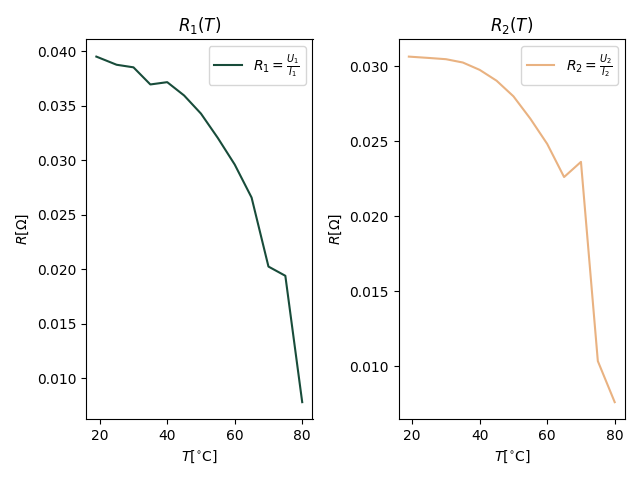
\includegraphics[width=.9\linewidth]{figures/r_od_T.png}
\end{center}
\caption{\small Graf prikazuje odvisnost ohmske upornosti $R(T)$}
\end{slika}

\subsection{Graf \(R_H (T)\)}\label{sec:org1e5d2b3}

Po enačbi \ref{eq:1} lahko z znanima \(c = 0.95 \mathrm{mm}\) in \(B = 0.173 \mathrm{T}\) izračunamo \(R_H\) pri različnih temperaturah in s tem dobimo željeni graf.

\begin{slika}[H]
\begin{center}
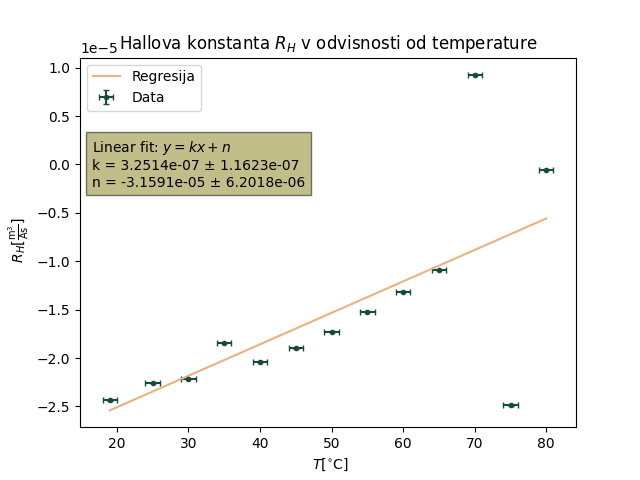
\includegraphics[width=.9\linewidth]{figures/hallovaKonstanta.png}
\end{center}
\caption{\small Graf prikazuje odvisnost Hallove konstante $R_{H}$ od temperature. Vidno je, da narašča z višanjem temperature.}
\end{slika}

Graf načeloma ustreza regresiji, razen pri predpredzadnjem členu, kjer je meritev podatkov nanesla, da je tok \(U_2\) bil večji od \(U_1\) in posledično je bila razlika pozitivna. Tudi v nadaljni obravnavi mi je to povzročalo težave, saj sem imel tako negativno vrednost v logaritmu, česar pa v realnem prostoru ne znamo izračunati.

\subsection{Graf logaritma gostote nosilcev naboja v odvisnosti od \(\frac{1}{k_B T}\)}\label{sec:org895ea45}

S pomočjo enačbe \ref{eq:1} lahko zapišemo enačbo

\[ \ln{n} = \ln \left( - \frac{IB}{U_H c e_0} \right)
\]

To na graf narišemo v odvisnost od \(\frac{1}{k_B T}\) in prilagodimo dve premici na dobljeno krivuljo. Dobil sem vrednosti

\begin{align*}
  E_g &\approx (0.65 \pm 0.03) \mathrm{eV} \\
E_D &\approx (0.17 \pm 0.03) \mathrm{eV}
\end{align*}

\begin{slika}[H]
  \centering
  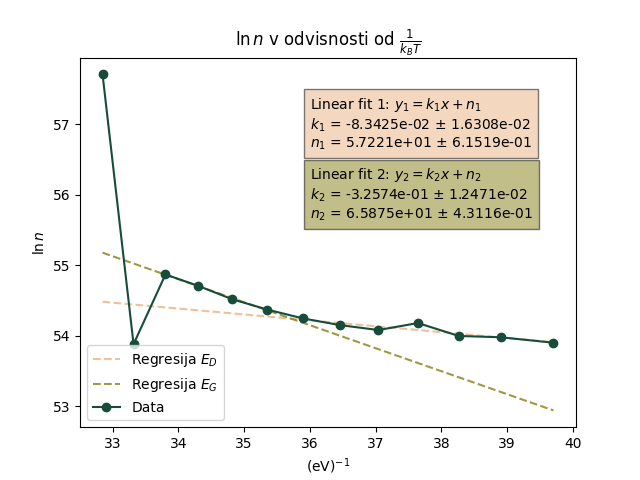
\includegraphics[width=.9\linewidth]{figures/logaritemgraf.png}
  \caption{\small Graf prikazuje odvisnost gostote nosilcev naboja v odvisnsto od $\frac{1}{k_{B}T}$. Z izmerjenimi podatki sem imel težave, saj so bili nekje celo negativni (kar ne gre skupaj z logaritmom). Dobro bi bilo ponoviti meritve v okolici višjih temperatur.}
\end{slika}

V skladu z literaturo omenjeno v razdelku \ref{sec:orgb97d12e} se podatki za donorsko režo drastično razlikujejo. Energijska reža pa se ujema z literaturo.


\section{Komentar}\label{sec:org24f504a}

Vaja je bila načeloma uspešna, je pa potrebno omeniti drastično različen rezultat donorske reže od literature. Prav tako so se močno poznale napake pri meritvi.

Smiselno bi bilo v okolici visokih temperatur meritve znova opraviti, da bi razrešili, kaj se je tu zalomilo.
\end{document}
